In this sub-section, we present details of implementation of the 
kernel modules (\texttt{pdatadump}, and \texttt{preadwritedump}) 
as well as the userspace tool (\texttt{psiphon}).

\subsection{Trace file format to enable correct parsing}
The output trace files generated by this toolkit are to be eventually
used for replay in the \textit{simreplay} simulator, described earlier.
Thus, all the elements of the previous trace format were retained in 
our format as well, albeit in a different ordering. Especially, the 
entire binary dump of the content per request was done, instead of 
dumping only the MD5 hash of the content. However, the most important
difference introduced is that because of the arbitrary nature of binary
characters, it was no longer feasible to simply use any ASCII character
as a delimiting character across the elements of each trace. 

Usually, a delimiting character is picked such that it is itself not
part of any of the fields within the record. Since the content dump
could be arbitrary (i.e., we can not control it), we could no longer
rely on a delimiting character to help parse/differentiate distinct
elements of a single trace file. The workaround identified is to 
indicate the beginning of each record using a special struct, namely
\texttt{struct trace\_event\_element}. The definition of this struct
is presented below in Listing \ref{lst:trace-event-element}.

\lstset{language=C,
	caption={Data-structure indicating the beginning of a record in
		trace files.},
	label=lst:trace-event-element
}
\begin{snippet}
struct trace_event_element
{
    __u32 magic;
    __u32 elt_len;  /* length of data in next trace element */
};
\end{snippet}

As is shown, struct \texttt{trace\_event\_element} consists of two 
entities: (i)~\textit{magic}, and (ii)~\textit{elt\_len}. The 
\textit{magic} value is a fixed value defined within the module, such
that if the defined value does not match the value in the trace file,
a parsing error can be declared. The second entity is basically a value
that reports the number of bytes following this structure, to form 
the rest of the current record. Thus, based on the value of \texttt{elt\_len},
those many bytes can be read from the trace file, and considered as a
single record. Within every single record, the binary content field is
always the last field and hence, the delimiter for all of the previous
fields is still retained as a blank space. Consequently, after the 
second-to-last field has been parsed, it can be safely assumed that 
remaining buffer content is itself the binary content dumped as part 
of the current trace record.

\subsection{Using relay channels with debugfs to dump output logs}
As mentioned in the previous section, we use relay channels and
debugfs to dump output logs from the kernel module, and use another
userspace module to siphon the logs from debugfs into persistent
storage repository. Using the \texttt{relaychan\_init()} call, we
create relay channels per CPU with name \textit{pioevents}, such 
that a file named \textit{pioevents.i} is created within 
\texttt{debugfs} for each CPU core numbered \textit{i}. For 
example, if the VM has two vCPUs, two files named \textit{pioevents.0}
and \textit{pioevents.1} would be created. This is done during
kernel module initialization, so that immediately after initialization,
the relay channels would be ready for use.

Once the kernel module is in use, it will keep intercepting disk
read and write requests and dumping relevant output into the
relay channels. Note that, depending on which CPU is processing
the disk request, the corresponding relay channel file will be
written into. For example, events processed by CPU-0 will cause
output to be written into \textit{pioevents.0} file whereas those
processed by CPU-1 will have output written into 
\textit{pioevents.1} file,
and so on. Thus, our entire trace would be split up into multiple
trace files when dumped via the relaychannel subsystem. Because
we eventually want to obtain a single trace file at a later time, 
we also print a timestamp for each event that is logged. After the
tracing is complete and the logging has been terminated, we
use the timestamps to merge all the output files and get an
integrated timestamp-ordered output trace file.

\subsection{Difference between \texttt{pdatadump} and \texttt{preadwritedump}}
As mentioned earlier, the \texttt{pdatadump} module dumps data content
only for write requests, and not for read requests. This is because, 
it also has another kernel thread running parallelly that performs a 
``scan'' of the entire disk and outputs per-block content into another 
relay channel. Thus, for all read requests, the corresponding content
is expected to be gather separately by the ``scanning thread'' of the
\texttt{pdatadump} module. Consequently, the \texttt{pdatadump}
module operates two relay channels, while the \texttt{preadwritedump}
module operates just one.

In \texttt{pdatadump}, since content needs
to be dumped only for write requests, and not read requests, only a
single-point probe/intervention is sufficient to gather the requisite
information, i.e. the \texttt{jprobe} at \texttt{generic\_make\_request}.
This is because at this probe point, the I/O requests are just being queued
for execution, and at this time, the read buffers are empty while 
the write buffers contain data. The read buffers are populated only
after execution, in the return path, at which time, the write buffers
have already been consumed (and potentially even reused elsewhere).
Thus, using a single probe, either the read content or the write content
can be dumped, not both. Hence, the \texttt{pdatadump} module makes
the choice of dumping content only for the write requests, %and not the reads,
while simultaneously ``scanning'' all the blocks to gather remaining content.

The advantage of the approach in \texttt{pdatadump} module is that, it
simplifies the design of the kernel module itself. 
However, the disadvantage of this approach is that, usage of the 
collected traces for replay becomes slightly unwieldy than if the read 
request content had also been present along-with. More specifically,
the absence of data content along-with the read request implies that
simulated disk ``creation'' had to be performed using the ``scanning''
traces, in advance of performing each simulated replay invocation.
Moreover, the ``scanning'' traces could be huge due to large size
storage capacity, even if the actual content being read may only
be a fraction of the total size~\cite{iodedup}.
With this in mind, we soon graduated to the newer implementation of
the kernel module, i.e. the \texttt{preadwritedump} module.

As mentioned above, dumping the data content only for write requests
enabled the implementation of the kernel module to be relatively simple.
However, since our new requirement is to dump the data content for
read requests as well, we adopted a similar approach as was done in
the \texttt{collect} kernel module (this was the incomplete source code
received from authors of \cite{iodedup}, mentioned earlier).
The idea is that for a read request that has been queued up to be 
associated with the corresponding completed read request, we need to
do some stacking and un-stacking of function pointers. This requires
in-kernel manipulation of I/O buffers of type \texttt{struct bio},
as explained next.

\subsection{Using jprobes to capture disk read and write requests}
In both \texttt{pdatadump} and \texttt{preadwritedump}, read and write
requests are intercepted by using a \texttt{jprobe} of the following form,
shown in Listing~\ref{lst:jprobe}.
\lstset{language=C,
	caption={The jprobe defined within the kernel module, to intercept disk read and write requests},
	label=lst:jprobe
}
\begin{snippet}
static struct jprobe jp_make_request = {
    .kp.addr = (kprobe_opcode_t *) generic_make_request,
    .entry = (kprobe_opcode_t *) my_make_request
};  
\end{snippet}


\lstset{language=C,
	caption={The structure for \texttt{oldbio}, similar to original \texttt{struct bio} of the Linux kernel},
	label=lst:oldbio
}
\begin{snippet}
struct old_bio_data_prwd {
  void          *bi_private;    //to stow away the original struct bio
  bio_end_io_t  *bi_end_io;	    //pointer to original bi_end_io()
  sector_t      bi_sector;	    //starting sector of data being requested
  unsigned      bi_size;        //size of the data being requested
  dev_t         bd_dev;		    //device of data being requested
  unsigned      major;		    //major number of device
  unsigned      minor;		    //minor number of device
  unsigned      pid;   		    //process id of the current process
  char          processname[PNAME_LEN];	//process name of above process
};
\end{snippet}

During kernel module initialization, the above jprobe is registered
using \texttt{register\_jprobe()} so that for every disk read and write
request, the call to \texttt{my\_make\_request} would be invoked, hence
giving us access to its \texttt{struct bio} arguments.
Thus, \texttt{my\_make\_request()} is our jprobe handler, and for a write
request, it dumps the
write content as well as identifying information into a relay channel.
However, the behaviour of the \texttt{jprobe} handler when encountering
a read request, is slightly modified. Instead of immediately dumping
to a relay channel, the handler simply notes the identifying information
in a newly-defined \texttt{struct oldbio} which is quite similar to
the original \texttt{struct bio} (refer Listing~\ref{lst:oldbio}). 
Additionally, the actual dumping of
content and identifying information for a read request is delegated 
to a separate function call, namely \texttt{bio\_end\_prwd()}. 

Originally, the I/O completion routine is the \texttt{bi\_end\_io} call w
which is invoked for each \texttt{bio} that is ready for consumption.
However, to associate the ``queue'' and ``completion'' events for the
various read requests, the original function pointer for \texttt{bi\_end\_io}
is stowed away into \texttt{struct oldbio}, whereas the function pointer
for \texttt{bio\_end\_prwd()} is ``stacked'' into the original 
\texttt{struct bio} in its place. This causes our new routine 
\texttt{bio\_end\_prwd()} to be invoked first during read I/O completion,
at which time, the dumping of read content happens. At the end of the
\texttt{bio\_end\_prwd()} routine, we invoke the original \texttt{bi\_end\_io}
so that read I/O execution can complete as usual.

\subsection{Exit handshake between kernel module and userspace process}
\begin{figure}[t]
    \centering
    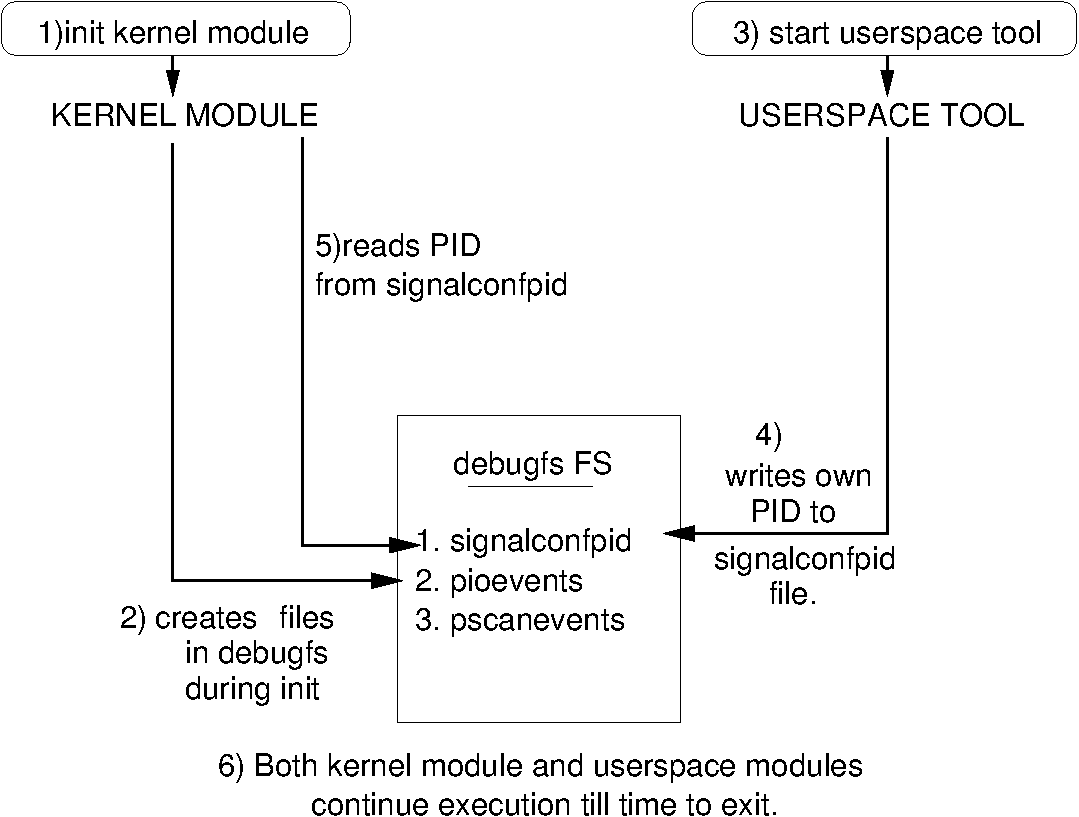
\includegraphics[scale=0.65]{tracingchap-figures/tracing-handshakesetup.pdf}
%    \vspace{-0.1in}
    \caption{Exit handshake setup: 
		\textit{Setting up for the exit handshake between the kernel 
		module and the userspace process involves writing of self PID
		into a \texttt{debugfs} file by the userspace process. The other
		two files listed here are the \texttt{debugfs} output files 
		of the kernel module.}}
    \label{fig:tracing-handshakesetup}
%    \vspace{-0.2in}
\end{figure}

\begin{figure}
    \centering
    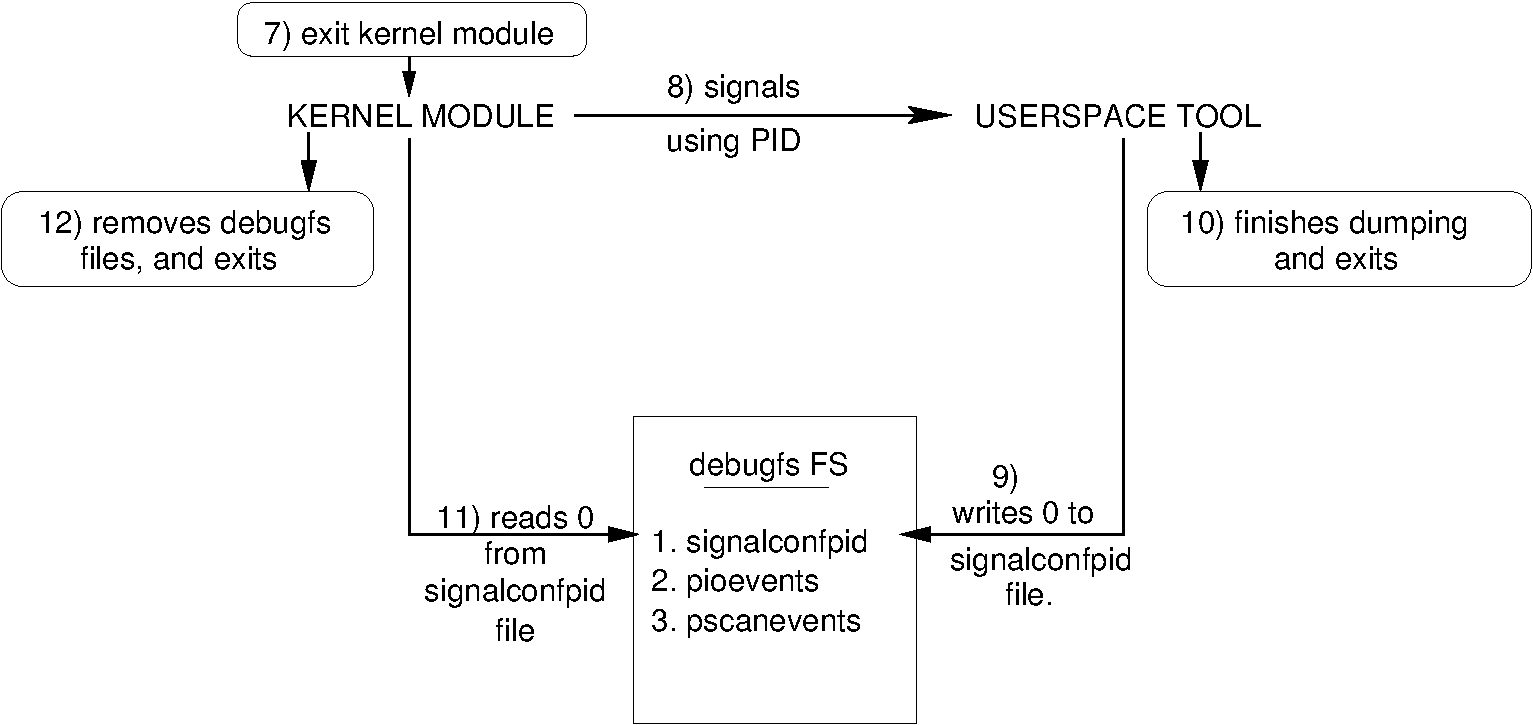
\includegraphics[scale=0.65]{tracingchap-figures/tracing-exithandshake.pdf}
%    \vspace{-0.1in}
    \caption{\textit{Execution of the exit handshake between the kernel
		module and the userspace process.}}
    \label{fig:tracing-exithandshake}
%    \vspace{-0.2in}
\end{figure}

Fig. \ref{fig:tracing-handshakesetup} shows the setup for performing the
signaling from the kernel to the userspace process. As mentioned earlier,
this requires that the kernel module is aware of the PID of the userspace
process. As shown in the figure, when the kernel module is init-ed, 
it creates a file named \texttt{signalconfpid} in the \texttt{debugfs} 
filesystem, in addition to other files for relay channels. After the
kernel module has been installed, the userspace tool is instantiated
and it determines its own process ID (PID) to write to the 
\texttt{signalconfpid} file. When the kernel module detects that a PID
has been written, it notes the value in local memory for future use.
After this initial exchange of PID, both the kernel module and the
userspace tool continue their trace dumping \& collection process, until
the kernel module requires to be un-installed. The actual handshake
to achieve graceful exit is performed when the kernel module is 
un-installed, as explained next.

\subsection{Executing the exit handshake}
Signaling is used so that after the kernel stops dumping output to the 
relay channels, it can notify the userspace process. An exit handshake is
accomplished which ensures that the data being logged has been captured
in its entirety. Fig. \ref{fig:tracing-exithandshake} presents the
handshake performed between the two modules, before the kernel module exit.
Upon receiving the signal from the kernel module, 
the userspace process finishes transferring any remaining data from 
the \texttt{debugfs} file system to the regular files, and exits. However, 
before exiting, the userspace program indicates its exit to the kernel
module by over-writing the previous PID value with zero. Upon receiving
a value of zero (0), the kernel module can safely exit.

